
\section{Language Hyper-Heuristic with \our{}}\label{sec: reevo}

LHH takes COP specifications as input and outputs the best inductive heuristic found for this COP.
Vanilla LHH can be repeated LLM generations to randomly search the heuristic space, which is sample-inefficient and lacks reasoning capabilities for complex and black-box problems (see \cref{sec: evaluating reevo}). Therefore, we propose Reflective Evolution (\our{}) to interpret genetic cues of evolutionary search and unleash the power of LHHs. 

\our{} is schematically illustrated in \cref{fig: reevo}. Under an evolutionary framework, LLMs assume two roles: a \textit{generator LLM} for generating individuals and a \textit{reflector LLM} for guiding the generation with reflections. \our{}, as an LHH, features a distinct individual encoding, where each individual is the code snippet of a heuristic. Its evolution begins with population initialization, followed by five iterative steps: selection, short-term reflection, crossover, long-term reflection, and elitist mutation. We evaluate the meta-objective of all heuristics, both after crossover and mutation. Our prompts are gathered in \cref{app: prompts}.

\begin{figure}[h!]
\begin{subfigure}{\textwidth}
    \centering
    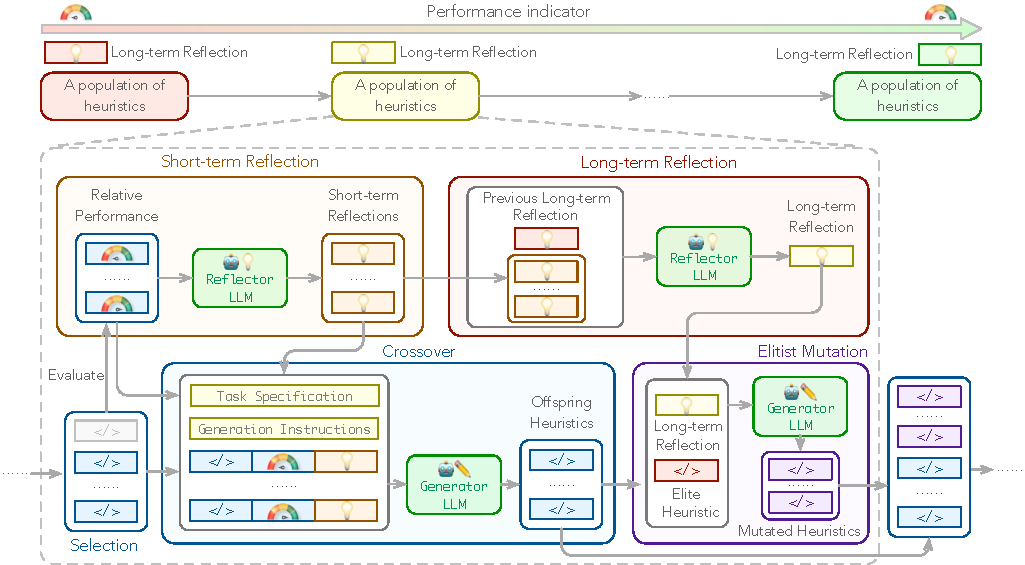
\includegraphics[width=1.0\textwidth]{figures/reevo_v4_compressed.pdf}
    % \vskip -0.05in
    \caption{\our{} pipeline. \textbf{Top}: \our{} evolves a population of heuristics. Insights and knowledge are verbalized as long-term reflections and accumulated throughout iterations. \textbf{Bottom}: A \our{} iteration contains five sequential steps: selection, short-term reflection, crossover, long-term reflection, and elitist mutation.}
\end{subfigure}
% \vskip 0.05in
\begin{subfigure}{\textwidth}
    \centering
    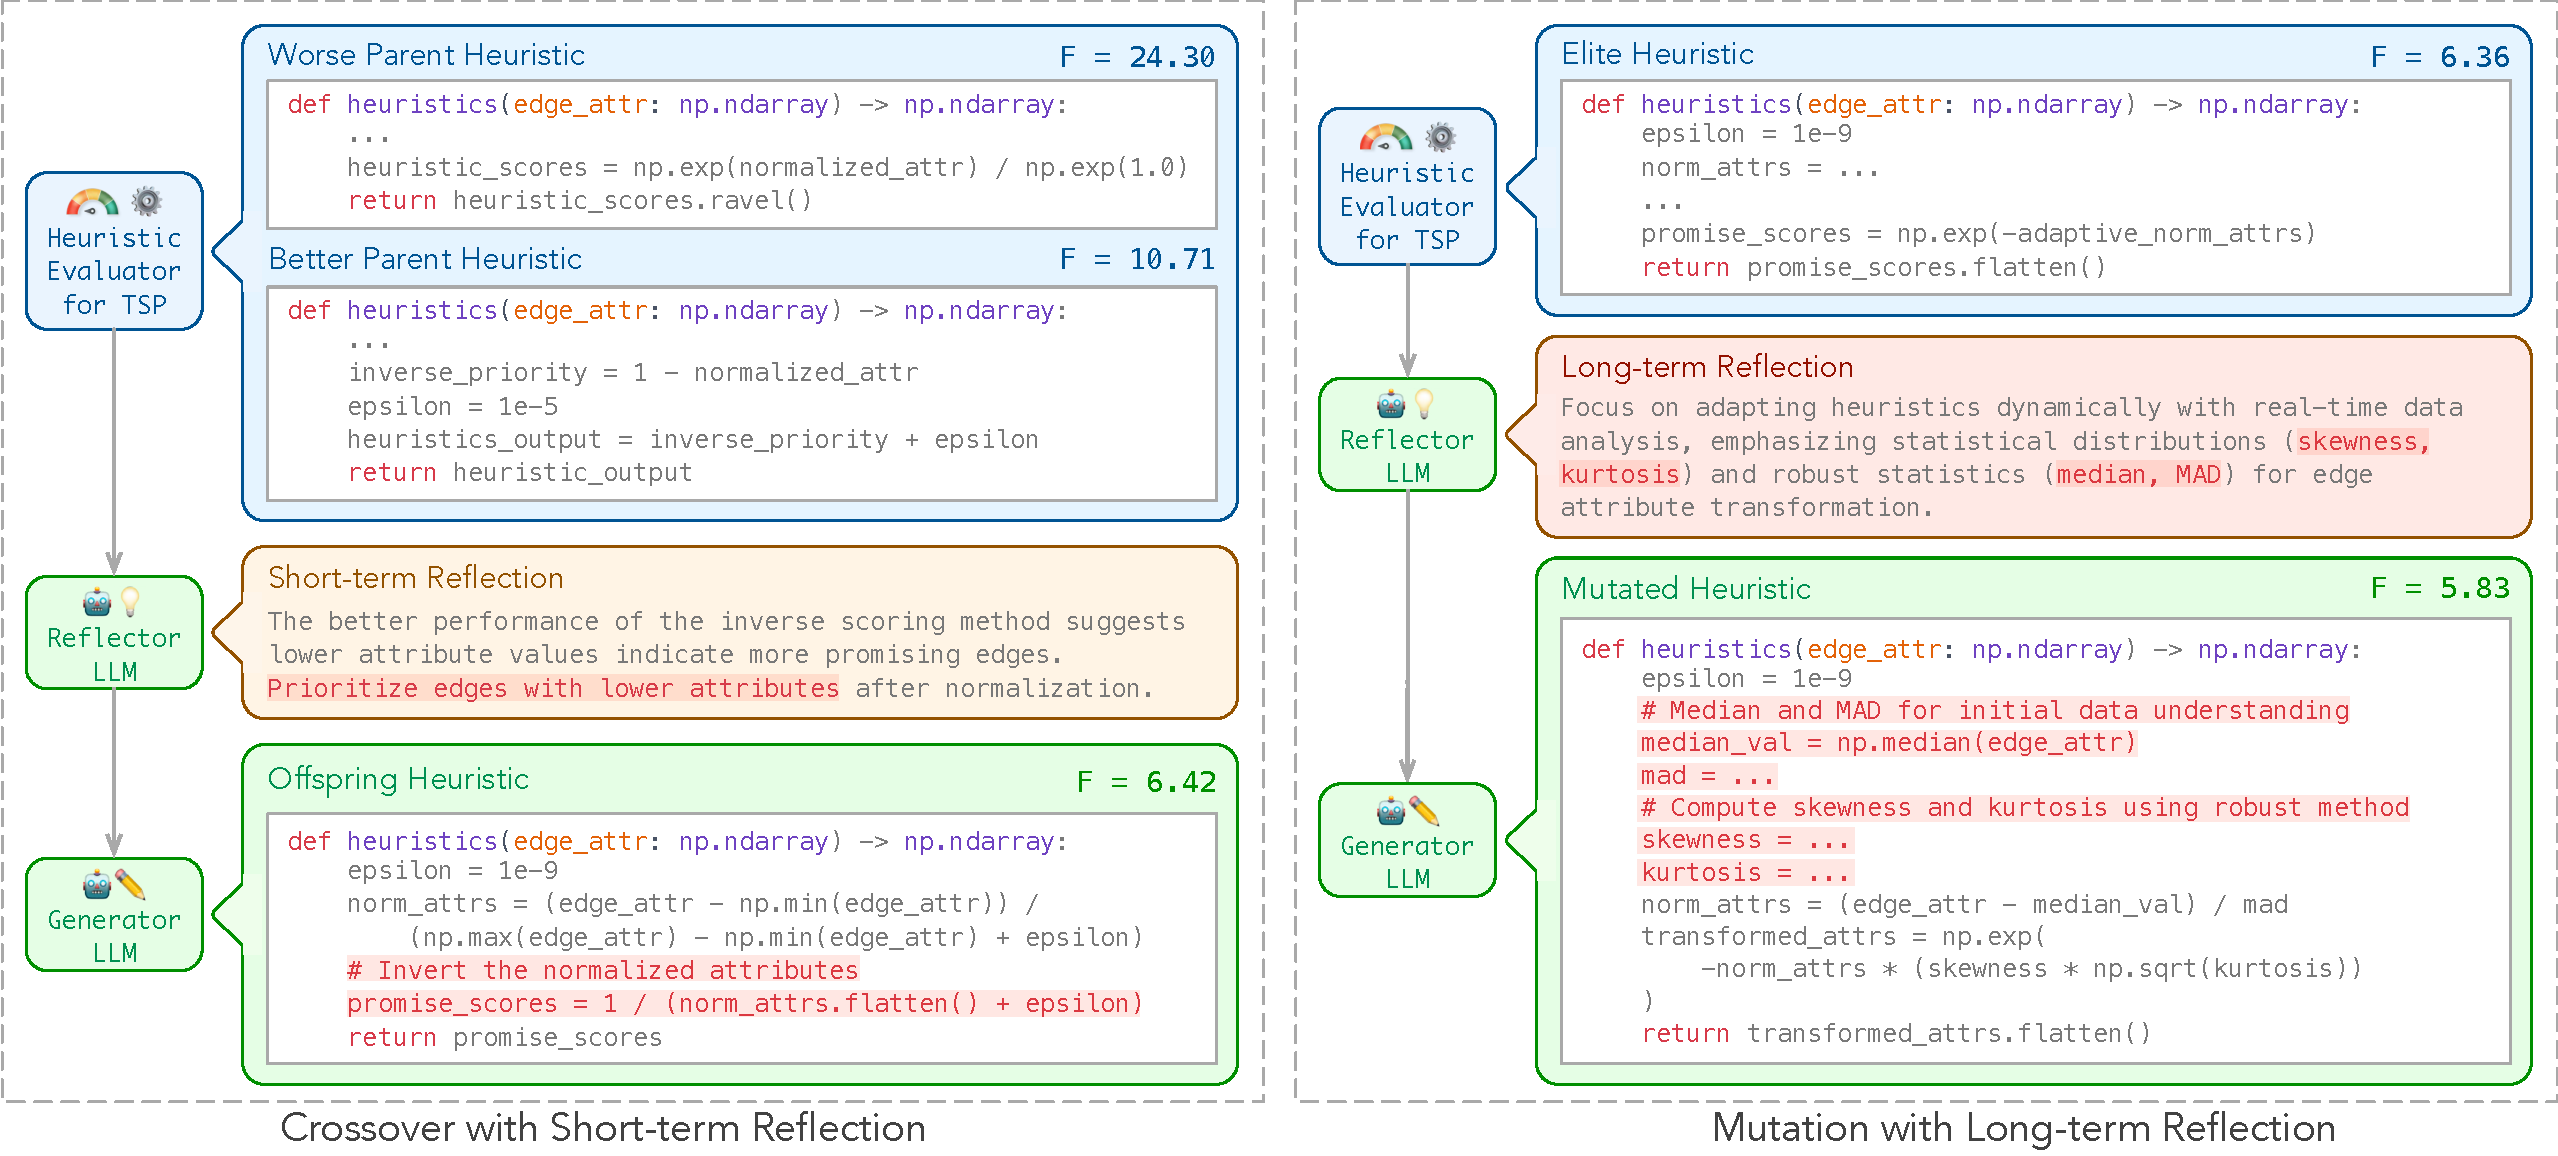
\includegraphics[width=1.0\textwidth]{figures/show_reflec_v3.pdf}
    % \vskip -0.05in
    \caption{Examples of reflections for black-box TSP. Heuristics are designed for Ant Colony Optimization (see \cref{sec: heuristic measures for aco}). \textbf{Left}: Given a pair parent heuristics, \our{} correctly infers the TSP objective and generates a better offspring accordingly. \textbf{Right}: Given the elite heuristic and accumulated long-term reflections, \our{} incorporates the suggested statistics and yields a better mutated heuristic.}
\end{subfigure}
\vskip -0.05in
\caption{An illustration of \our{}.}
\label{fig: reevo}
\end{figure}


\paragraph*{Individual encoding. }\our{} optimizes toward best-performing heuristics via an evolutionary process, specifically a Genetic Programming (GP). It diverges from traditional GPs in that (1) individuals are code snippets generated by LLMs, and (2) individuals are not constrained by any predefined encoding format, except for adhering to a specified function signature.


\paragraph*{Population initialization. }\our{} initializes a heuristic population by prompting the generator LLM with a task specification. A task specification contains COP descriptions (if available), heuristic designation, and heuristic functionality. Optionally, including seed heuristics, either trivial or expertly crafted to improve upon, can provide in-context examples that encourage valid heuristic generation and bias the search toward more promising directions.

A \our{} iteration contains the following five sequential steps.

\paragraph*{Selection. }\our{} selects parent pairs from successfully executed heuristics at random, while avoiding pairing heuristics with an identical meta-objective value \(F\). 

\paragraph*{Short-term reflection. } For each pair of heuristic parents, the reflector LLM reflects upon their relative performance and gives hints accordingly for improved design.
Unlike prior work \cite{shinn2023reflexion}, \our{} integrates the reflections into evolutionary search and reflects by performing comparative analyses. Our proposed approach is analogous to interpreting genetic cues and providing verbal gradients within search spaces, which leads to smoother fitness landscapes and better search results (see \cref{sec: fitness landscape analysis}).

\paragraph*{Crossover. }\our{} prompts the generator LLM to generate an offspring heuristic, given task specifications, a pair of parent heuristics, explicit indications of their relative performance, short-term reflections over the pair, and generation instructions.

\paragraph*{Long-term reflection. }\our{} accumulates expertise in improving heuristics via long-term reflections. The reflector LLM, given previous long-term reflections and newly gained short-term ones, summarizes them and gives hints for improved heuristic design.


\paragraph*{Elitist mutation. }\our{} employs an elitist mutation approach. Based on long-term reflections, the generator LLM samples multiple heuristics to improve the current best one. A mutation prompt consists of task specifications, the elite heuristic, long-term reflections, and generation instructions.

Viewing \our{} from the perspective of an LLM agentic architecture \cite{xi2023_llm_agents_survey}, short-term reflections interpret the environmental feedback from each round of interaction. Long-term reflections distill accumulated experiences and knowledge, enabling them to be loaded into the inference context without causing memory blowups.